\immediate\write18{makeindex Thesis.nlo -s nomencl.ist -o Thesis.nls}
%%
%% This is file `hustthesis-zh-example.tex',
%% generated with the docstrip utility.
%%
%% The original source files were:
%%
%% hustthesis.dtx  (with options: `example-zh')
%%
%% This is a generated file.
%%
%% Copyright (C) 2013-2014 by Xu Cheng <xucheng@me.com>
%%               2014-2016 by hust-latex <https://github.com/hust-latex>
%%
%% This work may be distributed and/or modified under the
%% conditions of the LaTeX Project Public License, either version 1.3
%% of this license or (at your option) any later version.
%% The latest version of this license is in
%%   http://www.latex-project.org/lppl.txt
%% and version 1.3 or later is part of all distributions of LaTeX
%% version 2005/12/01 or later.
%%
%% This work has the LPPL maintenance status `maintained'.
%%
%% The Current Maintainer of this work is hust-latex Organization.
%%
%% This work consists of the files hustthesis.bst, hustthesis.dtx,
%% hustthesis.ins and the derived file hustthesis.cls
%% along with its document and example files.
%%
%% \CharacterTable
%% {Upper-case    \A\B\C\D\E\F\G\H\I\J\K\L\M\N\O\P\Q\R\S\T\U\V\W\X\Y\Z
%%  Lower-case    \a\b\c\d\e\f\g\h\i\j\k\l\m\n\o\p\q\r\s\t\u\v\w\x\y\z
%%  Digits        \0\1\2\3\4\5\6\7\8\9
%%  Exclamation   \!     Double quote  \"     Hash (number) \#
%%  Dollar        \$     Percent       \%     Ampersand     \&
%%  Acute accent  \'     Left paren    \(     Right paren   \)
%%  Asterisk      \*     Plus          \+     Comma         \,
%%  Minus         \-     Point         \.     Solidus       \/
%%  Colon         \:     Semicolon     \;     Less than     \<
%%  Equals        \=     Greater than  \>     Question mark \?
%%  Commercial at \@     Left bracket  \[     Backslash     \\
%%  Right bracket \]     Circumflex    \^     Underscore    \_
%%  Grave accent  \`     Left brace    \{     Vertical bar  \|
%%  Right brace   \}     Tilde         \~}
\documentclass[format=draft,language=english,degree=phd]{hustthesis}
\usepackage{nomencl, epigraph, booktabs}
\renewcommand{\nomgroup}[1]{
%\ifthenelse{\equal{#1}{A}}{\item[\textbf{Roman Symbols}]}{%
\ifthenelse{\equal{#1}{G}}{\item[\textbf{Greek Symbols}]}{%
\ifthenelse{\equal{#1}{C}}{\item[\textbf{Abbreviations}]}{%
\ifthenelse{\equal{#1}{U}}{\item[\textbf{Superscripts}]}{%
\ifthenelse{\equal{#1}{S}}{\item[\textbf{Subscripts}]}% matches mathematical symbols
}% matches Greek Symbols
}% matches Abbreviations
}% matches Superscripts
}% matches Subscripts
}% matches Roman Symbols
\makenomenclature

\stuno{D201277241}
\schoolcode{10487}
\title{太阳能光热梯级发电系统设计\\及其特性研究}{Cascade solar thermal power system design and research of the key features}
\author
{张成}{Zhang Cheng}
\major
{热能工程}{Thermal Engineering}
\supervisor
{高伟\hspace{0.5em}教授\hspace{1em} Inmaculada Arauzo\hspace{0.5em}教授}{Prof. Gao Wei \newline Prof. Inmaculada Arauzo}
\date{2017}{6}{1}

\zhabstract{
    随着化石能源的消耗和环境问题的凸显,太阳能作为一种新能源,具有分布广泛、总量巨大、取之不竭、无污染的特点,越来越受到世界各国的重视,被广泛认为是未来最有潜力替代传统化石能源的清洁能源。在发电领域,太阳能光热发电是除了太阳能光伏发电之外的另一种发电形式,与光伏发电相比,光热发电因具有发电平稳,电网兼容性友好,易于与现有化石燃料电厂组合等优点而受到越来越多的关注。

    本课题属于国家国际合作项目专项“太阳能梯级集热发电系统关键技术合作研究”,本项目的目标是研究太阳能高温集热装置,提出并组建、优化太阳能梯级集热发电系统。本项目针对各种传统型式的太阳能光热发电系统的优缺点,为探索出可大规模低成本利用太阳能的光热发电技术提供新的方案。本课题通过建立各部件的机理模型,选择合理的拓扑结构,组建太阳能光热梯级集热发电系统,并建立系统的模型,针对不同的优化目标选择优化参数进行优化,最终得到低成本高效率的太阳能光热梯级发电方案,为实现高效率太阳能极热发电和大规模低成本应用提供技术支持。

    首先,针对太阳能光热梯级集热发电系统的各部件建立机理模型。依据目标对象的运行机理,根据物理平衡方程,对系统中的各部件,尤其是系统中的关键部件,建立起数学模型。各部件的数学模型是经由经典理论或是大量实验数据验证的模型,是组建光热梯级集热发电系统模型的基础。其次,提出了多种太阳能光热梯级系统的拓扑结构。通过热力学分析,结合系统中各部件的工作特点,合理布局太阳能光热梯级集热发电系统,利用不同热功循环实现不同品位的能量的梯级利用。
}
\zhkeywords{槽式集热器,碟式集热器,朗肯循环,斯特林循环,斯特林机组,梯级发电}

\enabstract
{
    With the increasing awareness of problem of fossil energy consumption and environmental pollution, solar energy as a renewable energy, which has the advantages as widely spreeded, huge amount, inexhaustible, no pollution, has received much attention by many countries and been regarded as the greated potential candidate of the fossil energy. Concentrated solar thermal power generation is another form of power generation technology except solar photovoltaic power generation. Compared to solar photovoltaic, solar thermal power is gaining more attention for its advantages as smooth power generation, good grid compatibility, easy to combinate with existing fossil power plant.

    The project of this research is an international cooperation program 'Collaborative research on key technologies to produce electricity by cascade utilization solar thermal energy'. The objective of the project is to investigate the key scientific problems related to solar heat collector in high temperature, cascade utilization solar thermal energy with high efficiency, system integration and optimizaition to develop the prototype system.
}
\enkeywords
{Parabolic trough collector, Parabolic dish collector, Rankine cycle, Stirling cycle, Stirling engine array, cascade powering}

\begin{document}

\frontmatter
\maketitle
\makeabstract
\tableofcontents
\printnomenclature
\listoffigures
\listoftables
\mainmatter

\chapter{Introduction}\label{chapter:Introduction}
\epigraph{Saving our planet, lifting people out of poverty, advancing economic growth... these are one and the same fight. We must connect the dots between climate change, water scarcity, energy shortages, global health, food security and women's empowerment. Solutions to one problem must be solutions for all.}{\textit{Ban Ki-moon}}

This dissertation considers a way to solve the global problems of energy shortage and environment problem.

\section{Solar Parabolic Trough}\label{sec:pt}

Parabolic trough solar technology is the most proven and lowest cost large-scale solar power technology available.~\cite{Price2002}

Figure~\ref{fig:pt} shows a parabolic trough product made by Alpha-E.

\begin{figure}[!ht]
\centering
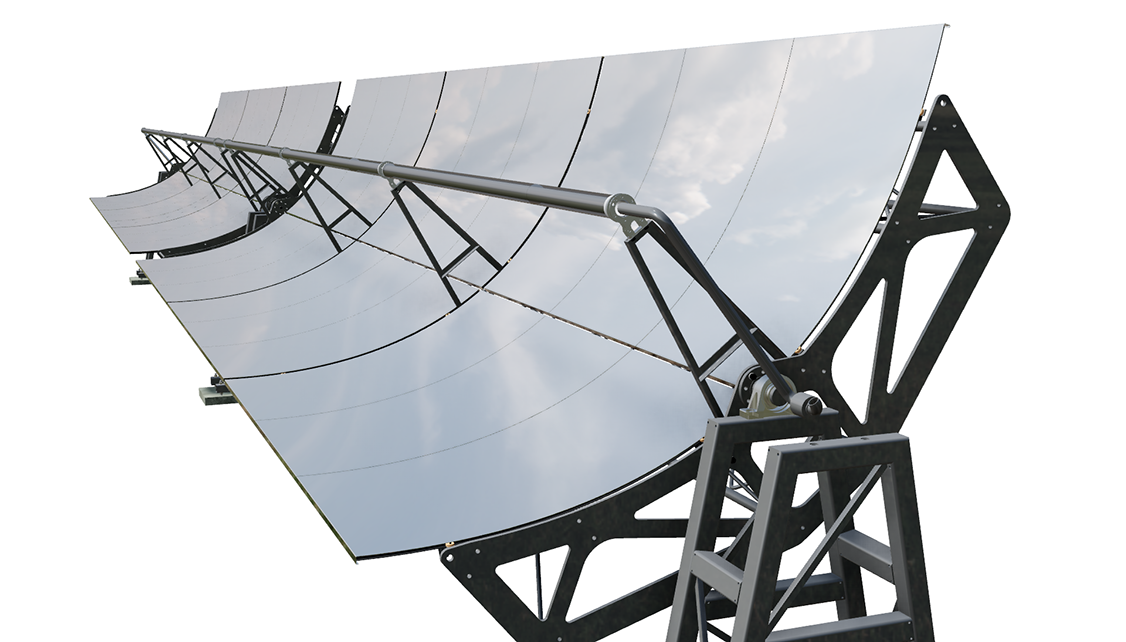
\includegraphics[width=.7\textwidth]{fig/ParabolicTrough.png}
\caption{Alpha-Trough-350, a parabolic trough product made by Alpha-E}\label{fig:pt}
\end{figure}

Padilla~\cite{Padilla2011} performed a detailed one dimensional numerical heat transfer analysis of a PTC (Parabolic Trough Collector).  To solve the mathematical model of heat transfer of the PTC model, the partial differential equations were discretized and the nonlinear algebraic equations were solved simultaneously. The numerical results was validated to the data from Sandia National Laboratory (SNL).
\nomenclature[C]{PTC}{Parabolic Trough Collector}
\nomenclature[C]{SNL}{Sandia National Laboratory}

To understand the thermal performance of the collector and identify the heat losses from the collector, Mohamad~\cite{Mohamad2014} analyzed the temperature variation of the working fluid, tube and glass along the collector.

Guo~\cite{JiangfengGuo2016-1} investigated the energy efficiency and exergy efficiency of the parabolic trough collector. The result shown that there exists an optimal mass flow rate of working fluid for exergy efficiency, and the thermal efficiency and exergy efficiency have opposite changing tendencies under some conditions.

Guo~\cite{JiangfengGuo2016-2} implemented a multi-parameter optimization of parabolic trough solar receiver based on genetic algorithm where Exergy and thermal efficiencies were employed as objective function.

Padilla~\cite{Padilla2014} performed a comprehensive exergy balance of a parablic trough collector based on the previous heat transfer model~\cite{Padilla2011}. The results shown that inlet temperature of heat transfer fluid, solar irradiance, and vacuum in annulus have a significant effect on the thermal and exergetic performance, but the effect of wind speed and mass flow rate of heat transfer fluid is negligible. It was obtained that inlet temperature of heat transfer fluid cannot be optimized to achieve simultaneously maximum thermal and exergetic efficiency because they exhibit opposite trends. Finally, it was found that the highest exergy destruction is due to the heat transfer between the sun and the absorber while for exergy losses is due to optical error.

Huang~\cite{Huang2012} proposed an analytical model for optical performance which employed a modified integration algorithm.

Wang~\cite{Wang2016} proposed a mathematical model for the optical efficiency of the parabolic trough solar collector and selected three typical regions of solar thermal utilization in China for the model. The model is validated by comparing the test results in parabolic trough power plant, with relative error range of 1\% to about 5\%.

Al-Sulaiman~\cite{AlSulaiman2014} presented the exergy analysis of selected thermal power systems driven by PTSCs. The power pf the thermal power system is produced using either a steam Rankine cycle (SRC) or a combined cycle, in which the SRC is the topping cycle and an organic Rankine cycle (ORC) is the bottoming cycle.
\nomenclature[C]{SRC}{Steam Rankine Cycle}
\nomenclature[C]{ORC}{Organic Rankine Cycle}

Hachicha~\cite{Hachicha2013} presented a detailed numerical heat transfer model based on the finite volume method for the parabolic trough collector.  This model is based on finite volume method and ray trace techniques and takes into account the finite size of the Sun.  The model is thoroughly validated with results from the literature and it shows a good agreement with experimental and analytical results.

Ashouri~\cite{Ashouri2015} coupled a small scale parabolic trough collector and a thermal storage tank along with an auxiliary heater to a Kalina cycle to study the performance of the system throughout the year, both thermodynamically and economically.

Guo~\cite{SuGuo2016} developed a nonlinear distribution parameter model to model the dynamic behaviors of direct steam generation parabolic trough collector loops under either full or partial solar irradiance disturbance.

Bader~\cite{Bader2015} developed a numerical model of a tubular vavity-receiver that uses air as the heat transfer fluid. Four different receiver configurations are considered, with smooth or V-corrugated absorber tube and single- or double-glazed aperture window. The different types of energy loss by the collector have been quantified, and the temperature distribution inside the receiver has been studied. The pumping power required to pump the HTF through the receiver has been determined for a 200 m long collector row.

Good~\cite{Good2015} proposed solar trough concentrators using air as heat transfer fluid at operating temperatures exceeding 600$^\circ$C. It consists of an array of helically coiled absorber tubes contained side-by-side within an insulated groove having a rectangular windowed opening. Secondary concentrating optics are incorporated to boost the geometric concentration ratio to 97$\times$.

Boukelia~\cite{Boukelia2016} investigated the feed-forward back-propagation learning algorithm with three different variants; Levenberge Marguardt (LM), Scaled Conjugate Gradient (SCG), and Pola-Ribiere Conjugate Gradient (PCG), used in artificial neural network (ANN) to find the best approach for prediction and techno-economic optimization of parabolic trough solar thermal power plant (PTSTPP) integrated with fuel backup system and thermal energy storage.
\nomenclature[C]{LM}{Levenberge Marguardt}
\nomenclature[C]{SCG}{Scaled Conjugate Gradient}
\nomenclature[C]{PCG}{Pola-Ribiere Conjugate Gradient}
\nomenclature[C]{ANN}{Artificial Neural Network}
\nomenclature[C]{PTSTPP}{Parabolic Trough Solar Thermal Power Plant}

Kaloudis~\cite{Kaloudis2016} investigated a PTC system with nanofluid as the HTF in terms of Computational Fluid Dynamics (CFD). Syltherm 800 liquid oil was used as the HTF, and Al$_2$O$_3$ nanoparticles with the concentrations ranges from 0\% to 4\% was investigated. A boost up to 10\% on the collector efficiency was reported for Al$_2$O$_3$ concentration of 4\%.
\nomenclature[C]{HTF}{Heat Transfer Fluid}
\nomenclature[C]{CFD}{Computational Fluid Dynamics}

Tan~\cite{Tan2014} proposed a two-stage photovoltaic thermal system based on solar trough concentration is proposed, in which the metal cavity heating stage is added on the basis of the PV/T stage, and thermal energy with higher temperature is output while electric energy is output. The experimental platform of the two-stage photovoltaic thermal system was established, with a 1.8 m$^2$ mirror PV/T stage and a 15 m$^2$ mirror heating stage, or a 1.8 m$^2$ mirror PV/T stage and a 30 m$^2$ mirror heating stage. The results showed that with single cycle, the long metal cavity heating stage would bring lower thermal efficiency, but temperature rise of the working medium is higher, up to 12.06$^\circ$C with only single cycle. With 30 min closed multiple cycles, the temperature of the working medium in the water tank was 62.8$^\circ$C, with an increase of 28.7$^\circ$C, and thermal energy with higher temperature could be output.

Al-Sulaiman~\cite{AlSulaiman2012} proposed a nvel system based on PTC and ORC for combined cooling, heating and power (CCHP). Performance assessment, including efficiency, net electrical power, and electrical to heating and cooling ratios, of the system shown that when CCHP is used, the efficiency increases significantly. This study reveals that the maximum electrical efficiency for the solar mode is 15\%, for the solar and storage mode is 7\%, and for the storage mode is 6.5\%. The maximum CCHP efficiency for the solar mode is 94\%, for the solar and storage mode is 47\%, and for the storage mode is 42\%.
\nomenclature[C]{CCHP}{Combined cooling, heating and power}

Lobon~\cite{Lobon2014} introduced a computational fluid dynamic simulation approach to predict the behavior of a solar steam generating system, which is located at the Plataforma Solar de Almeria, Spain. The CFD package STAR-CCM+ code has been used to implement an efficient multiphase model capable of simulating the dynamics of the multiphase fluid in parabolic-trough solar collectors. Numerical and experimental data are compared in a wide range of working conditions.
\nomenclature[C]{DSG}{Direct Steam Generation}

Xu~\cite{Xu2014} presented a method to compensate the end loss effect of PTC. An optical analysis on the end loss effect of PTC with horizontal north-south axis (PTC-HNSA) is performed and a five-meter PTC-HNSA experimental system was built. The increased thermal efficiency of the experimental system is measured, and the result that the experimental value (increased thermal efficiency) substantially agreed with the theoretical value (increased optical efficiency) is gained.

Liu~\cite{Liu2012} developed a mathematical model of PTC using the least squares support vector machine (LSSVM) method. Numerical simulations are implemented to evaluate the feasibility and efficiency of the LSSVM method, where the sample data derived from the experiment and the simulation results of two solar collector systems with 30 m$^2$ and 600 m$^2$ solar fields, and the complicated relationship between the solar collector efficiency and the solar flux, the flow rate and the inlet temperature of the heat transfer fluid (HTF) is extracted.
\nomenclature[C]{LSSVM}{Least squares support vector machine}

\section{Solar Parabolic dish}\label{sec:pd}

One of the main goals of the BIOSTIRLING-4SKA project, funded by the European Commission, is the development of a hybrid Dish-Stirling system based on a hybrid solar-gas receiver, which has been designed by the Swedish company Cleanergy.~\cite{Blazquez2016}

Craig~\cite{Craig2016} proposed two types of cooking sections of the solar parabolic dish system: the spiral hot plate copper tube and the heat pipe plate. A conical cavity of copper tubes were put on the focus of the collectors to collect heat and the heat is stored inside an insulated tank which acts both as storage and cooking plate. The use of heat pipes to transfer heat between the oil storage and the cooking pot was compared to the use of a direct natural syphon principle which is achieved using copper tubes in spiral form like electric stove. An accurate theoretical analysis for the heat pipe cooker was achieved by solving the boiling and vaporization in the evaporator side and then balancing it with the condensation and liquid-vapour interaction in the condenser part while correct heat transfer, pressure and height balancing was calculated in the second experiment. The results show and compare the cooking time, boiling characteristics, overall utilisation efficiencies and necessary comparison between the two system and other existing systems.

Flux distribution of the receiver is simulated successfully by Mao~\cite{Mao2014} using MCRT method. The impacts of incident solar irradiation, aspect ratio (the ratio of the receiver height to the receiver diameter), and system error on the radiation flux of the receiver are investigated.
\nomenclature[C]{MCRT}{Monte Carlo Ray Tracing}

Mawire~\cite{Mawire2014} 40~m$^2$ 40 m$^2$

An experimental setup to investigate the thermal performance of a cylindrical cavity receiver for an SK-14 parabolic dish concentrator is presented in this technical note. The thermal performance is evaluated using energy and exergy analyses. The receiver exergy rates and efficiencies are found to be appreciably smaller than the receiver energy rates and efficiencies. The exergy factor parameter is also proposed for quantifying the thermal performance. The exergy factor is found to be high under conditions of high solar radiation and under high operating temperatures. The heat loss factor of the receiver is determined to be around 4.6 W/K. An optical efficiency of around 52% for parabolic dish system is determined under high solar radiation conditions. This experimental setup can be used as teaching tool for people with little or no knowledge about solar dish concentrators due its simplicity and the basic mathematical formulations applied. Different types of receivers and different types of deep focal region parabolic dishes can also be tested with the experimental setup.

\section{Solar Tower}\label{sec:st}
\section{Rankine Cycle}\label{sec:rc}
\section{Stirling Engine}\label{sec:se}
\section{Brayton Cycle}\label{bc}
\section{Research Objective}\label{sec:3}

\chapter{System Design}

\section{System Structure}
\section{Component Modeling}
Object oriented method is used for system modeling.
%\subsection{Solar Field}
\subsection{Solar Parabolic Trough}
\subsection{Solar Parabolic Dish}
\subsubsection{Solar Dish Collector}
\subsubsection{Solar Dish Receiver}
\subsection{Steam Generators}
\subsection{Power Block}
\subsection{Condenser}
\subsection{Deareator}
\subsection{Stirling Engine}
\subsection{Heat Storage System}


\chapter{System Analysis}

\section{Energy Cascade Collection}

\section{Energy Cascade Utilization}


\begin{table}[htbp]
  \centering
	\caption{Parameters of SEA models}
	\begin{tabular}{cc}
		\toprule
		Parameters	&	Value\\
		\midrule
		$s_{se}$	&	20 Hz\\
		$U_hA_h$	&	180 W/K\\
		$U_cA_c$	&	180 W/K\\
		$n_{se}$	&	6\\
		$q_{m,h}$	&	0.3 kg/s\\
		$q_{m,c}$	&	0.3 kg/s\\
		%$T_{i,h}$	&	1000 K\\
		%$T_{i,c}$	&	300 K\\
		$P_{i,h}$	&	5$\times$10$^5$ Pa\\
        $P_{i,c}$	&	5$\times$10$^5$ Pa\\
		\bottomrule
	\end{tabular}
	\label{tab:parameters}
\end{table}
\nomenclature{$s$}{Speed of Stirling enine, Hz}
\nomenclature[S]{$se$}{Stirling engine}
\nomenclature[U]{$'$}{Separate system}

\section{Stirling Engine Array}

\section{Steam Generators}

\chapter{Conclusions}

\backmatter

\begin{ack}
  This is the acknowledgement part.
\end{ack}

\bibliography{bib/bibliography.bib}

\appendix

\begin{publications}

  \item Zhang Cheng, Kun Wang. International Conference on Power Engineering: ICOPE 2013: FEA simulation on the alignment of the shafts of three-fulcrum turbine.
  \item Performance comparison of new and traditional arrangements of a dish-Stirling system
	\item A multi-stage exergy-loss reduction system for solar parabolic trough power plants
	\item Cascade system using both trough system and dish system for power generation

  \item A solar thermal cascade system, No. 201610806296.5
  \item A flow control method used in a multi-stage heating system, No. 201610805604.2

\end{publications}

\chapter{Formulae}\label{appendix:2}
  The is the content of the Appendix B

\end{document}

\endinput
%%
%% End of file `thesis.tex'.
